\section{Problema 4: Puzzle de casilleros}

\subsection{Introducci\'on}

\quad Para este tipo de problemas, se suele usar la t\'ecnica de \textit{backtracking}. No se conocen algoritmos polinomiales para resolver el problema. Tambi\'en se podr\'ia resolver con fuerza bruta pero la ventaja de esta t\'ecnica es que se busca armar e ir probando posibles soluciones. A medida de que se van construyendo, se puede determinar ciertos casos que no son posible soluci\'on, por lo que no se intentar\'ia resolver el problema en esos casos evitando ejecuciones innecesarias. En el peor caso, \textit{backtracking} es igual a intentar resolverlo por fuerza bruta.
\quad Se nos pide encontrar, si existe, alguno de los menores subconjuntos de piezas de tal forma que cubran todo el tablero. Donde cada casillero del tablero es de color negro o blanco, y cada pieza de forma rectangular, posee casilleros de los mismos colores. La pieza para poder ubicarse en cierta posici\'on del tablero tiene que coincidir exactamente en el tablero y se la puede rotar. 

\subsection{Desarrollo}

\quad Este ejercicio contiene varios problemas. Para empezar, nos encontramos con el requerimiento de dado un conjunto armar todos los subconjuntos posibles. Se conoce como \textit{power set}. La complejidad de este problema es exponencial, no se conocen algoritmos polinomiales hasta el momento.

\quad La primera implementaci\'on del problema de power set consist\'ia en usar una m\'ascara de bits para determinar si un elemento estaba presente o no en un conjunto. Se recorr\'ian los n\'umeros desde el 1 hasta $ 2^{ \vert piezas\vert} $ formando as\'i todas las posibles combinaciones de subconjuntos. Era simple pero ten\'ia el problema de que pod\'ia producir overflow en arquitecturas donde ${\vert piezas\vert} $ sea mayor a la cantidad m\'axima de bits para alg\'un registro que sea utilizado como contador del procesador. Ej: con 40 piezas y un procesador de 32 bits.

\quad Por lo tanto, decidimos implementar este problema mediante la recursi\'on.


%\quad Para resolver el problema principal, lo que hicimos fue ir probando cada uno de los subconjuntos con tama\~no desde 1 hasta la %cantidad de piezas. Como punto de corte razonable, es haber encontrado alg\'un subconjunto como soluci\'on.

\quad Lo primero que hace el algoritmo antes de comenzar a probar con ubicaciones es realizar una poda. Esta primera poda que se realiza es para descartar piezas que no podrían ubicarse en ninguna parte del tablero. Por ejemplo, en un caso extremo, si el tablero es completamente negro, una pieza con alguna parte blanca no puede ubicarse y por lo tanto no podría pertenecer jamás a la solución. Esta primera poda es clave, porque ya desde el principio nos evitamos analizar ramas que no son solución del problema.

\quad Una vez eliminadas estas piezas, se prosigue buscando todos los subconjuntos del conjunto de piezas, es decir se calcula el conjunto de partes (o powerset) del conjunto de piezas. De esta manera obtenemos todas las combinaciones posibles de las piezas que no fueron descartadas hasta el momento. A continuación, ordenamos el conjunto de partes, poniendo en primer lugar a los subconjuntos de menor cantidad de elementos.

\quad Luego, se iterará sobre la cantidad de subconjuntos, y apenas se encuentre una solución se dejará de ciclar y se la devolverá. Como el conjunto está ordenado, se garantiza de esta manera que se encontró la solución con la menor cantidad de piezas, que es la que queríamos devolver (esto es porque todos los conjuntos que se evaluaron antes no solucionaron el problema).


\quad Para determinar si cierto subconjunto de piezas es soluci\'on, determinamos una nueva poda. Esta consiste en que, al buscar una soluci\'on \'optima, el subconjunto de piezas debe de cubrir exactamente el tablero. Si la superficie de las piezas del subconjunto es menor al del tablero, entonces no puede ser soluci\'on porque no cubriría el tablero. En cambio, si es mayor, podr\'ia ser soluci\'on, pero si lo era, no era \'optima porque sobraba alguna pieza.



\quad Luego implementamos una funci\'on recursiva en la cual para cada pieza se busca sus posibles posiciones en el tablero. Para cada posici\'on, se crea una instancia del tablero en la cual se ubica dicha pieza. Luego se llama recursivamente a la funci\'on con ese tablero y sin esa pieza.

\quad El caso base de la funci\'on es cuando no quedan m\'as piezas por ubicar. Entonces se chequea si el tablero est\'a completamente cubierto, en caso afirmativo, se encontr\'o una soluci\'on al problema.

\quad La funci\'on tiene en cuenta las rotaciones de las piezas. Por lo que si no se encontr\'on soluci\'on, se rota la pieza. Si es id\'entica a la original, se poda esa rama. Caso contrario, se busca todas las posibles posiciones para esa pieza rotada, y se repite lo anterior.

\quad Una vez que se encuentra soluci\'on, si existe, se devuelve el vector con la informaci\'on de las piezas colocadas en el tablero. \'Este vector, lo maneja la clase \textit{Tablero} que hicimos, al cual agrega una pieza cada vez que es posible ubicarla en el tablero.

\quad En todo momento del desarrollo tuvimos que tener en cuenta generar todas las podas posibles para evitar ejecuciones innecesarias debido al tipo de problema.

\quad Creamos las clases \textit{Tablero} y \textit{Pieza} para que cada se encargue de las funciones que les competen propiamente a dicha abstracci\'on. 

\quad En la clase \textit{Tablero}, podemos crear un tablero con el tama\~no deseado, obtener las posibles posiciones de una pieza, si encaja la pieza en cierta posici\'on, si est\'a completo o no. Si cierto conjutno de piezas puede llegar a cubrir todo el tablero, obtener las piezas ubicadas, etc.

\quad En la clase \textit{Pieza}, podemos crear una pieza de cierto tama\~no, rotarla, etc.

\quad Utilizamos top-down y clases porque nos pareci\'o la mejor forma de organizar el programa para resolver el ejercicio. Haciendo m\'as prolijo el c\'odigo y \textit{tirar} los problemas del tablero se encarga su clase y el de la pieza el de ella misma.



\subsubsection{Correctitud}

%\quad En cuanto la problema de la generaci\'on de todos los subconjuntos posibles de un conjunto, utilizamos un m\'etodo que dada la representaci\'on binaria de un n\'umero los elementos presentes en un conjunto son aquellos donde la posici\'on es igual al id del elemento y el bit est\'a en 1, es decir, es un elemento presente. Como se recorre desde el valor 1 hasta $ 2^{n} $ (n es cantidad de elementos), se recorre todas las posibles  combinaciones de elementos presentes y no presentes. Si bien esta forma sigue siendo un algoritmo exponencial, creemos que es m\'as eficiente que haber hecho una funci\'on recursiva que genere todos estos conjuntos.

\quad Recorremos todas las posibles combinaciones de las fichas. Luego para cada subconjunto nos fijamos si es solución. En caso de existir solución, es esperable que esta supere todas las podas que hemos determinado. Es decir que el tamaño de la suma de las piezas del subconjunto coincide con el tablero y que cada pieza del subconjunto puede ubicarse en el tablero, que en el fondo son propiedades necesarias pero no suficientes que debe cumplir una solución. Es decir que no estamos podando piezas que podrían pertenecer al conjunto solución. Esta es la ventaja del backtracking, que se podría caractizar como fuerza bruta un poco más inteligente, al ahorrarse operaciones que no tiene sentido realizar. 
\quad Teniendo en cuenta que a lo mejor se nos escapó agregar alguna otra poda, lo que queremos remarcar es que estamos recorriendo subconjuntos que pueden o no ser solución y que recortamos ramas con potencial para serlo. De esta manera, aunque se pudiesen agregar podas, se estarían analizando todas las potenciales soluciones.

\quad Como además recorremos los subconjuntos de menor a mayor cantidad de elementos y dado que el algoritmo deja de iterar en los subconjuntos una vez que halle una solución, se está garantizando que la solución devuelta (en caso de exisir) es una solución óptima en el sentido de que se completa el tablero con la menor cantidad de piezas posibles, que es lo que efectivamente se debe devolver.
\quad 

\subsubsection{An\'alisis de complejidad}

Las funciones que utlizamos del tablero son:

\begin{itemize}

\item \textbf{getColor:} dada una posici\'on del tablero, devuelve el color, negro o blanco. Tiene un costo O(1) debido a que solo tiene que devolver un valor accediendo a una posici\'on de una matriz.

\item \textbf{posiblesPosiciones:} recorre todo el tablero, fij\'andose en cada posici\'on, si es posible ubicar la pieza ah\'i. Para esto llama a la funci\'on encaja. Guarda en un vector resultado las posiciones posibles de ubicar la pieza. La complejidad termina siendo la cantidad de posiciones del tablero (filas por columnas) iteraciones de la funci\'on encaja: O(filas * columnas * filasPieza * columnasPieza)

\item \textbf{encaja:} dada una pieza y una posici\'on, devuelve verdadero si es posible ubicar esa pieza en la posici\'on pasada por par\'ametro. Para esto, recorre toda la superficie de la pieza, por lo que cuesta O(filasPieza * columnasPieza)

\item \textbf{ocupado:} dada una posici\'on, devuelve si ya está ocupada por una pieza o no. Se tiene que acceder a una matriz, por lo que cuesta O(1).

\item \textbf{completo:} determina si el tablero est\'a totalmente cubierto por piezas. Para ello, tiene que recorrer todas las posiciones y llamar a la funci\'on ocupado. Tiene coste O(filas * columnas)

\item \textbf{ubicarFicha:} dada una pieza y una posici\'on modifica la instancia de tablero, seteando las posiciones correspondientes para considerarlas ocupadas. Adema\'a, guarda en un vector el id de la pieza, el grado de rotaci\'on de la misma, y la posici\'on del extremo superior izquierdo. Tiene un costo O(filasPieza * columnasPieza)

\item \textbf{obtenerPiezas:} la clase tablero guarda un vector con las piezas ubicadas en el mismo. Esta funci\'on devuelve una copia de ese vector. Tiene costo O(n) donde n es la cantidad de piezas.

\item \textbf{cubreTodo:} es una funci\'on para podar casos no posibles de ser soluci\'on como se explic\'o anteriormente. Calcula la superficie del tablero. Recorre todas las piezas, restando a la superficie del tablero la superficie de la pieza. Para cubrirlo exactamente tiene que quedar en 0. Caso contrario, se poda. Tiene un costo de O(n) donde n es la cantidad de piezas.

\end{itemize}

\indent Vistas estas consideraciones, analicemos la complejidad de $resolverJuego$.  Lo haremos en función de la cantidad de piezas.\\
\indent Primero hagamos una aclaración: si bien es cierto que muchas de la funciones que usa este métodos basan su complejidad en el tamaño de la pieza que está probando en ese momento, hemos decidido acotar la cantidad de filas de una pieza por la cantidad de filas del tablero y lo mismo para la cantidad de columnas. Esto es porque al momento de ejecutar $resolverJuego$ es esperable que todas las piezas que se analizan tienen dimensiones menores o iguales a las del tablero. Por lo tanto, la cota de complejidad que mostraremos en esta sección es quiźa burda.\\
\indent Para esta análisis definiremos $k$ como las dimensiones del tablero. Es decir que $k$ es la cantidad de filas del tablero por la cantidad de columnas del tablero.\\

\indent Como se puede observar, $resolverJuego$ es una función recursiva en la cantidad de piezas. En el caso en que la cantidad de piezas sea nula, lo único que se chequea es si el tablero está completo en tiempo O(k).
\indent Si, en cambio, quedan piezas por analizar, el algoritmo chequea si se puede agregar al tablero alguna de las rotaciones de la pieza y luego se llama recursivamente a la función pero sin esa pieza. En el peor caso, lo que puede ocurrir es que se tenga que chequear las cuatro rotaciones de la pieza.\\
\indent Adem\'as de llamarse recursivamente el algoritmo realiza algunas operaciones. Por cada rotaciones, se fija las posibles posiciones con un costo de $O(k*filasPieza*columnasPieza)$. Hemos dicho que vamos a acotar las filas y las columnas de la piezas por las del tablero. Luego, supongamos que buscar las posibles posiciones cuesta $O(k^{2})$.\\
\indent Copiar la pieza que vamos a analizar cuesta O(filasPiezas*columnasPieza) y lo mismo para calcular cada rotación. Con la cota que dijimos antes cada una de estas operaciones cuesta O(k). Notemos que en el peor caso para cada pieza habría que chequear las cuatro rotaciones.\\
\indent En el peor caso, las posibles posiciones de la pieza son todas las del tablero, es decir $k$. Se va a iterar en la cantidad de posibles posiciones.El costo de lo que está adentro del ciclo es O(k+ T(n-1)), siendo T(n-1) el costo de la siguiente llamada recursiva a la función.\\
\indent Es decir que el costo de una llamada a la función con cantidad de piezas no nulas es de $4*[k + k^{2} + k* (k+T(n-1))]$, o lo que es lo mismo:\\
$4*[k + k^{2} + k^{2} + k* T(n-1)]$\\

\indent Pasando en limpio de manera más formal:\\
\indent $T(0)=k$\\
\indent $T(n)=4*[k + k^{2} + k^{2} + k* T(n-1)]$\\

\indent Veamos más detenidamente $T(n)$:\\
\begin{center}
\indent $T(n)= T(n)=4*[k + k^{2} + k^{2} + k* T(n-1)] = 4*k + 4*k{2} + 4*k^{2} + 4*k * T(n-1)=$ \\

\indent $= 4*k + 4*k^{2} + 4*k^{2} + 4*k *[4*k + 4*k^{2} + 4*k^{2} + 4*k * T(n-2)]=$\\

\indent $=4*k + 4*k^{2} + 4*k^{2} + 4^{2}*k^{2} + 4^{2}*k^{3} + 4^{2}*k^{3}+ 4^{2}*k^{2} * T(n-2)=$\\

\indent $=4*k + 4*k^{2} + 4*k^{2} + 4^{2}*k^{2} + 4^{2}*k^{3} + 4^{2}*k^{3}+ 4^{2}*k^{2} * [4*k + 4*k^{2} + 4*k^{2} + 4*k* T(n-3)]=$\\

\indent $=4*k + 4*k^{2} + 4*k^{2} + 4^{2}*k^{2} + 4^{2}*k^{3} + 4^{2}*k^{3}+ 4^{3}*k^{3} + 4^{3}*k^{4} + 4^{3}*k^{4} + 4^{3}*k^{3} * T(n-3)=$\\

\indent $=....=$\\

\indent $=  (4*k)^{n} * T(0) + \sum_{i=1}^{n} (4*k)^{i} + 2 * (4^{i}* k^{i+1})=$ \\

\indent $=  (4*k)^{n} * k + \sum_{i=1}^{n} (4*k)^{i} + 2 * (4^{i}* k^{i+1})$ \\

\end{center}


\indent Es decir que :\\

\indent $T(0)=k$\\
\indent $T(n)= 4^{n}* k^{n+1} + \sum_{i=1}^{n} (4*k)^{i} + 2 * (4^{i}* k^{i+1})$\\

\indent Conjeturamos que esto cuesta $O(4^{n}*k^{n+1})$. Veámoslo por inducción:\\

\indent Queremos ver que existe un $d$ real positivo y $n_{0}$ natural positivo tales que para todo $n\geq n_{0}$ vale que $T(n) \leq d * 4^{n}*k^{n+1}$.\\
\indent Caso base: n=1 \\

\begin{center}
\indent  $T(1)=4* k^{2} + 4*k + 2 * 4* k^{2} \leq 4* k^{2} + 4*k^{2} + 2 * 4* k^{2} \leq 4* (4*k^2)$\\
\indent Es decir que para $n=1$ considerando un $d \geq 4 $ alcanza.\\
\end{center}

\indent Paso inductivo: Supongo  que $T(n-1) \leq  d * 4^{n-1}* k^{n}$. Quiero ver que esto implica que  $T(n) \leq  d * 4^{n}* k^{n+1}$\\

\begin{center}

\indent $T(n)= 4*k + 4*k{2} + 4*k^{2} + 4*k * T(n-1) \leq 4*k + 4*k{2} + 4*k^{2} + 4*k * 4^{n-1}* k^{n} \leq $\\

\indent $\leq 4*k + 4*k{2} + 4*k^{2} + 4*k * 4^{n-1}* k^{n} \leq 4*k + 4*k{2} + 4*k^{2} + 4^{n}* k^{n+1} \leq $ \\

\indent $\leq 4^{n}*k^{n+1} + 4^{n}*k{n+1} + 4^{n}*k^{n+1} + 4^{n}* k^{n+1} \leq 4* 4^{n}* k^{n+1}$\\

\indent que es lo que queriamos ver.\\
\end{center}


\indent Luego, $resolverJuego$ cuesta O($4^{n}*k^{n+1}$).\\

\indent Veamos ahora la complejidad de $buscarSol$.\\
\indent  Esta función lo que hace es llamar a $descartarPiezas$, que se encarga de eliminar del vector de piezas a aquellas que no podrían entrar en el tablero porque no coinciden con ningún área de este. Esta función se vale de la función de Tablero $cabe$ que chequea si una pieza en particular entra en el tablero y que tiene una complejida de O($k*filasPiezas*columnasPieza$). Acotándolo como mencionamos anteriormente nos queda O($k^{2}$).\\
\indent  Luego, $descartarPiezas$ cuesta O($n* k^{2} + n^{2}$).\\

\indent Además, se genera el power set del vector luego de descartar las piezas. En el peor caso, no se descartó ninguna pieza. Entonces generar el conjunto de partes tiene un costo de O($n * 2^{n}$).\\
\indent  Ordenar este subconjunto tiene un costo de O($n * 2^{n}$), que se obtiene de la cota O($2^{n} * log(2^{n})$) que cuesta ordenar un vector de $2^{n}$ elementos (que es la cantidad de elementos que tiene el conjunto de partes o power set).\\

\indent Luego, $buscarSol$ itera en la cantidad de elementos del conjunto de partes. En el peor caso dijimos que son $2^{n}$ subconjuntos. Por cada iteración se llama a $esSolucion$ que chequea si las piezas cubren todo el tablero con un costo de O(n). Si lo hacen se llama a $resolverJuego$.\\

\indent Es decir que $esSolucion$ tiene una complejidad de O($n + 4^{n}*k^{n+1}$), que es O($4^{n}*k^{n+1}$) puesto que $k$ es entero positivo.\\

\indent Luego la complejidad total de $esSolucion$, que es la función que resuelve el problema es O($n* k^{2} + n^{2} + n * 2^{n} + 4^{n}*k^{n+1}$). O lo que es lo mismo:\\

\indent O( $max [(n* k^{2} + n^{2} ) , ( $n * 2^{n}$ ) , ( $4^{n}*k^{n+1}$ ) ] ).\\
 
 

\subsection{Resultados}

\begin{figure}[H]
	\centering
	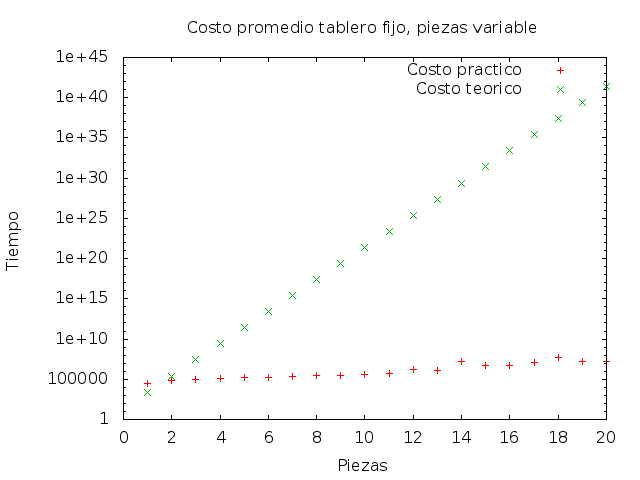
\includegraphics[scale=0.6]{ej4-grafico1.png}
	\caption{ En escala logar\'itmica}
\end{figure}

\begin{figure}[H]
	\centering
	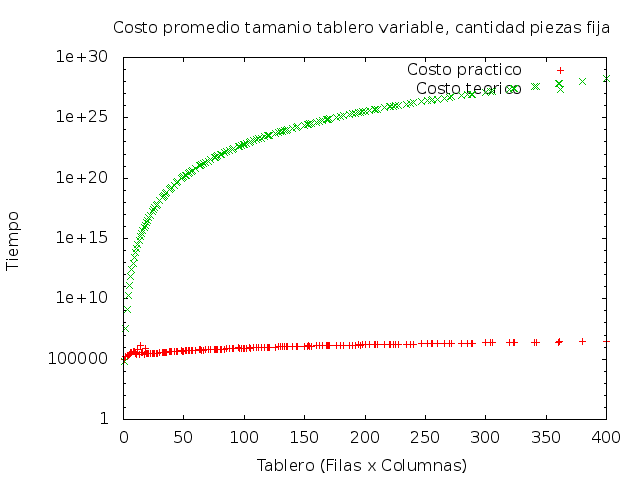
\includegraphics[scale=0.6]{ej4-grafico2.png}
	\caption{ En escala logar\'itmica}
\end{figure}



\subsection{Conclusiones}

\quad Considerando posibles mejoras ser\'ia que en vez de buscar \textit{linealmente} cual es la menor cantidad de piezas necesarias, se podr\'ia utilizar una busqueda binaria. Con linealmente nos referimos en el sentido de que probamos con una pieza, luego dos, y así sucesivamente hasta probar con todas las piezas. En cambio, con b\'usqueda lineal, se prueba con la mitad de piezas, si es soluci\'on, entonces existe una soluci\'on menor o igual a esa. Por lo que se busca una nueva soluci\'on entre la 1era mitad en cantidad de piezas. Sino, entonces era necesario m\'as piezas y se busca en la 2da mitad en cantidad de piezas.

\quad Hay que tener en cuenta que al ser un problema que no se resuelve polinomialmente, intentar resolver con un valor grande en cantidad de piezas puede demorar demasiado en comparaci\'on si se hubiese hecho b\'usqueda lineal. Si se pudiera hacer un estudio sobre las piezas y el tablero y se conociera una estad\'istica sobre la entrada del problema, se podr\'ia determinar casos donde conviene utlizar uno u otro.

\quad Con este problema, pudimos notar la importancia de determinar buenas podas o puntos de corte para tratar de realizar un backtracking eficiente. De esta forma, se puede llegar a resolver problemas dif\'iciles much\'isimo m\'as eficiente que si se hubiese realizado fuerza bruta.
